\documentclass{article}
\usepackage[utf8]{inputenc}
\usepackage{tikz}
\usepackage{amsmath}
\usepackage{float}
\usepackage{nips_2016}
\usepackage{txfonts}
\usepackage{bm}
\usepackage{amssymb}
\usepackage{mdwlist}
\usepackage{mathtools}
\usepackage[colorlinks]{hyperref}
\usepackage{float}
\usepackage{xfrac}
\usepackage{booktabs}
\usepackage{physics}
\usepackage{mdframed}
\usepackage{hyperref}
\usepackage{graphicx}
\usepackage{minted}
\usepackage{ mathrsfs }
\usepackage{wrapfig}
% http://tex.stackexchange.com/questions/5223/command-for-argmin-or-argmax#comment28205_5255
\DeclareMathOperator*{\argmin}{\arg\!\min}
\DeclareMathOperator*{\argmax}{\arg\!\max}

\newcommand{\abe}[1]{\textcolor{red}{AH: [#1]}}
\newcommand{\saul}[1]{\textcolor{blue}{SS: [#1]}}
%for displaying red texts
\usetikzlibrary{bayesnet,calc,patterns,angles,quotes,decorations.pathreplacing,bending,intersections}

\newcommand{\logitdeet}{\Bigg(\lg\frac{(L_{w_m}  B_{u_m} +  A_{u_m})}{1- \lg(L_{w_m}  B_{u_m} +  A_{u_m})}\Bigg)}

\newcommand\independent{\protect\mathpalette{\protect\independenT}{\perp}}
\def\independenT#1#2{\mathrel{\rlap{$#1#2$}\mkern2mu{#1#2}}}
\newcommand\given{\;\vert\;}

\newcommand\normal{\mathcal{N}}
\newcommand\logistic{\text{logistic}}
\newcommand\expected{\mathbf{E}}
\newcommand\data{\boldsymbol{\mathcal{D}}}
\renewcommand\thesubsection{\alph{subsection}}
\newcommand\me{\mathrm{e}}

\title{Project report: 697 StatML}
\author{Saul Shanabrook and Abram Handler}
\date{\today}

\begin{document}
\maketitle

\begin{figure}[h]
\begin{mdframed}
\includegraphics[width=13cm]{reuse3.png}
\centering
\caption{An example of ``text reuse'' in Congressional bills, displayed with a custom search tool built for this project (\S\ref{sec:future}). The passage occurs in two different bills from the 113th Congress. Green text was inserted during copying. Red text was deleted.}
\label{fig:example}
\end{mdframed}
\end{figure}

\section{Introduction}

Recent work in political science suggests that U.S. Congressional bills, traditionally imagined to be written by a single sponsor, sometimes contain passages from other legislation \cite{Wilkerson2013TracingTF}.

We are interested in modeling this ``text reuse'' to gain a better understanding of Congress. This project is a preliminary exploration. We (1) implement a computationally-efficient method for detecting repeating legislative text (2) develop and validate a model of the legislature (3) use the model to explore one aspect of text reuse in bills and (4) make plans for future work.

More concretely, in this preliminary study, we examine a simple question: do liberals in congress borrow text from ``conservative'' legislation? Do conservatives borrow from ``liberal'' legislation? Examining textual borrowing across party lines offers a new perspective on partisanship, at a finer level of detail than in traditional examinations of Congress. 


\section{Defining and detecting reuse in Congressional bills}

Congressional bills are divided into short numbered sections. We define ``text reuse'' as two bills which share a section with a Jaccard similarity greater than .8. This simple definition serves as useful starting place, although more complex definitions might be more useful in future work \footnote{For instance, any string of tokens of any length from any piece of legislation might be modified and copied into a different bill, regardless of section divisions. Moreover, changing some tokens within a string (e.g. a verb) will cause dramatic changes in meaning, while others (e.g. an adjective) likely do not. Finally, similar ideas such as ``cut taxes'' and ``reduce fees'' (a shared idea) can have entirely different textual forms. We will explore these alternate definitions in future work.}.

For this preliminary study, we downloaded 13,758 Congressional bills in bulk from Govtrak\footnote{\url{https://www.govtrack.us}} for the 113th Congress (2013--2014). We then used Govtrak's xml to divide the bills into 214,748 sections.

A naive all-pairs check of the Jaccard similarity of each section would require $214,748^2 \approx 4 * 10^{10}$  comparisons, which is intractable. Thus, to detect reuse, we implement the combination of ``minhashing'' and LSH-binning described in section 3.4.3 of \underline{Mining Massive Datasets} \cite{Rajaraman2011MiningOM}. The method, as described in detail in Leskovec \textit{et al.} \cite{Rajaraman2011MiningOM}, finds similar pairs with probability $p$, depending on configuration. We use 100 random permutations and a band size of 10 to find 367,613 possible pairs. We then check the actual word-type-level Jaccard similarity of each section and filter out those with a similarity less than .8 to create a final list of 232,619 pairs. Finally, we successfully generate the S-curve shown in figure 3.7 of \underline{Mining Massive Datasets}, using randomly generated data to confirm our implementation is working as specified\cite{Rajaraman2011MiningOM}.

\section{Modeling Congress with ideal point estimation}

We model legislative activity using ideal points, a technique from political science (see \S\ref{sec:related_work}). We assume that each of $K$ legislators has a real-valued ideology in one dimension, centered around 0. The $K$ legislators vote on $N$ bills\footnote{The same piece of legislation might have different versions as it moves through Congress, where it will be tagged with different metadata marking the text as introduced or as voted on. For now, we consider each version of a bill a separate bill.}. Each bill also has a real-valued ideology in one dimension centered around 0 and a real-valued bias centered around 0. The $K$ legislators cast $M$ votes on $N$ bills, where $M \approx K * N$ (ignoring missing votes). 

Intuitively, in our model, if a legislator's ideology is close to a bill's ideology, they will be more likely to vote yes on a bill. However, if a bill's bias is high, then the legislator will be more likely to vote yes on a bill, regardless of ideology. (Many bills are not controversial, such as naming post offices). Mathematically, this can be expressed as 

$$
V_m \sim \text{Bernouli}(p=\logistic(L_{w_m}  B_{u_m} +  A_{u_m}))
$$

where $L_{w_m}$ is the legislator casting vote $m$ and ($B_{u_m}, A_{u_m}$) is the bias and ideology of the bill being considered in vote $m$ (Table \ref{table:model}). For now, we only model yes and no votes, ignoring legislators who do not cast a vote on a given bill.

\begin{table}\label{table:model}
\centering
\begin{tabular}{llr}
\toprule
Symbol & Explanation \\
\midrule
L_k & \text{ideology of $k$th legislator} \\
B_n & \text{ideology of $n$th bill} \\
A_n  & \text{bias of $n$th bill} \\
w_m & \text{legislator who cast $m$th vote} \\ 
u_m & \text{bill considered in $m$th vote} \\
V_m \sim \text{Bernouli}(p=\logistic(L_{w_m}  B_{u_m} +  A_{u_m})) & \text{$m$th position} \\
\bottomrule
\end{tabular}
\caption{Model components}
\end{table}

%\begin{align*}
%    & L_k  &= \text{ideology of $k$th legislator} \quad &  k \in \{1, \ldots, K\} \\
%    & B_n &= \text{ideology of $n$th vote} \quad &  n \in \{1, \ldots, N\} \\
%    & A_n  &= \text{bias of $n$th vote} \quad & n \in \{1, \ldots, N\} \\
%    \\
%    & w_m &= \text{legislator of $m$th position} \quad & m \in \{1, \ldots, M\} \\
%    & u_m &= \text{vote of $m$th position} \quad & m \in \{1, \ldots, M\} \\
%    & V_m \sim \text{Bernouli}(p=\logistic(L_{w_m}  B_{u_m} +  A_{u_m})) 
%        &= \text{$m$th position} \quad & m \in \{1, \ldots, M\} \\
    \\
%\end{align*}

\begin{figure}[H]\label{fig:model}
\centering
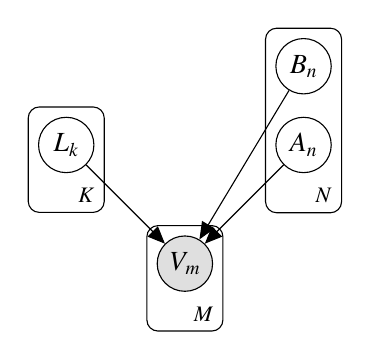
\begin{tikzpicture}
  
  \node[obs] (v) {$V_m$};
%   \node[const, above right = 2.0cm and 2.3cm of v] (w) {$\gamma$};
%   \node[const, above right = 1.0cm and 2.3cm of v] (x) {$\gamma$};
%   \node[const, above left = 1.0cm and 2.3cm of v] (z) {$\gamma$};
  %\node[latent, right=of v] (u) {$U_m$};

  \plate {} {(v) } {$M$} ;

  \node[latent, above left =1 cm and 1cm  of v] (l) {$L_k$};
  %  \node[latent,  right of b] (n) {$N_b$};
  \plate {} {(l)} {$K$} ;
  
  \node[latent, above right = 2cm and 1cm  of v] (b) {$B_n$};
  \node[latent, above right = 1cm and 1cm  of v] (a) {$A_n$};
  \plate{} {(a) (b)} {$N$} ;

%   \edge{w} {b};
%   \edge{x} {a};
%   \edge{z} {l};
  \edge {l, a, b} {v} ; %
\end{tikzpicture}
\caption{Our initial Bayesian model. $M$ votes are observed from $K$ legislators on $N$ bills. 

% $\gamma$ is a standard normal prior.
}
\end{figure}

Originally, we used a Bayesian model, treating the unknown ideologies and biases as latent variables, with standard normal priors (Figure \ref{fig:model}):%, denoted with $\gamma$ in the graphical model above:
\begin{align*}
    & L_k   \sim \normal(0, 1) \\
    & B_n  \sim \normal(0, 1) \\
    & A_n \sim \normal(0, 1)  \\
\end{align*}
To perform inference, we first used the PyMC3 Python package \cite{10.7717/peerj-cs.55}. It performs MCMC sampling in order to estimate the posterior distribution on the latent variables. It initializes this sampling with auto-diff variational inference (ADVI). The package returned reasonable ideal point estimates, but we found it to be too time-consuming as we increased the number of samples. We could have increased performance by performing learning on mini batches of data, but decided instead to focus on rewriting the learning from scratch.

In rewriting the inference procedure, we removed the priors on the latent variables to simplify the model and performed maximum likelihood estimation.

We started with randomly initialized parameters $\boldsymbol{\theta}$ all drawn from standard normal distributions and perform gradient ascent using these update equations. We include our work deriving gradients in \S\ref{sec:appendix}. We found that a learning parameter of $\alpha=0.003$ was a good trade off between training time and accuracy. If the learning parameter was too high the model would not converge.

We found the MLE learned similar ideal points to the sampling method, even though the likelihood function is not convex. It appears that local maximum for the log likelihood are good enough for our use case, or is in fact a global maximum.

\section{Validation}
We validated our model by visualizing the ideal points for legislators and votes. We checked these results against our intuition that Democrats and Republicans should have differing ideal points (Figure \ref{fig:ptleg}, \ref{fig:ptlegs}). Also, we found that less controversial bills have a higher bias, and that the ideologies of bills aligned with the parties that sponsored them (Figure \ref{fig:ptbills}). 

\begin{figure}[h]

    \begin{subfigure}
    \includegraphics[width=0.9\linewidth]{ptleg} 
    \caption{Learned ideal points of all legislators of the 113th Congress. Democrat and Republican legislators are clustered separately based on their ideologies.}
    \label{fig:ptleg}
    \end{subfigure}
    
    \begin{subfigure}
    \includegraphics[width=0.9\linewidth]{ptlegs}
    \caption{Ideal points for four well-known senators. The more moderate senators are closer to 0, while the more extreme are farther from 0.}
    \label{fig:ptlegs}
    \end{subfigure}
\end{figure}

\begin{figure}[h]
    \centering
    \includegraphics[width=0.9\linewidth]{ptbills} 
    \caption{Four bills, with ideal points and biases. The more conservative bills have ideal points below 0, and the more liberal have ideal points above 0. The Consolidated Appropriations Act, 2014 (a spending bill) has a neutral ideal point and  was approved by the majority of both parties.}
    \label{fig:ptbills}

\end{figure}

\section{Exploratory results}

Our preliminary investigation found many examples of text reuse that cross the liberal and conservative spectrum (Figure \ref{fig:reuse1}): that is passages which are copied from liberal bills into conservative bills and vice versa. However, the significance of these findings is not clear. Many examples of text reuse include boilerplate passages without obvious political import. For instance, unrelated bills might share the same standard paragraph detailing requirements for federal grants. We will need to split politically significant reuse from political boilerplate before we can build a model that better explains partisanship in Congress. 

\begin{figure}[h]
\centering
\begin{minipage}{.5\textwidth}
  \centering
  \includegraphics[width=6cm]{scatter.png}
  \label{fig:reuse1}
\end{minipage}%
\begin{minipage}{.5\textwidth}
  \centering
  \includegraphics[width=6cm]{hex.png}
  \label{fig:reuse2}
\end{minipage}
\caption{A scatter plot (left) of 1117 unique instances of text reuse in the 113th Congress, also shown as a hexbin (right). Each point on the scatter plot represents a passage shared between two bills. The ideal point of the first bill is shown on the x-axis, the ideal point of the second bill on the y-axis.
Note that of the 13,758 bills in the 113th congress, only 1,862 actually reach a floor vote, which is why so few detected pairs are shown. (Our model does not currently give ideal points for bills that do not reach a vote). Each section's ideal point is assumed to be the same as the ideal point for the overall bill, although this could be refined in future work.}
\end{figure}

Specifically, we note the following kinds of reuse. Some seem uninteresting and others seem worthy of further investigation.

\begin{itemize}
    \item \textbf{Appropriations changes} In some cases, legislators change the amount of an appropriation, as in figure \ref{fig:example}. These sorts of changes do reflect fine-grained political bargaining and might yield a better understanding of Congress.
    \item \textbf{Political insertions and deletions} In some cases, insertions and deletions are politically interesting. For instance, in one case, mention of a critical report from a government watchdog was deleted during copying. It is not clear how to split politically interesting edits from politically uninteresting edits (see \S\ref{sec:future})
    \item \textbf{Boilerplate} Some repeating sections are Congressional boilerplate. The passages appear in many bills, with small changes---as if legislators were filling in the blanks.
    \item \textbf{Non-political insertions and deletions} In some cases, legislators paraphrase while copying passages, often in ways which are not politically significant. For instance, ``United States'' might get rewritten as ``United States of America''.
    \item \textbf{Change of section number} In many cases, legislators copied whole passages, but changed a section number. 
\end{itemize}

\section{Related work}\label{sec:related_work}
Detecting text reuse and understanding Congressional partisanship are each well-studied topics. In the future, we hope to contribute by joining these strands of research. 

``Tracing the Flow of Policy Ideas in Legislatures'', from Wilkerson, Smith and Stramp \cite{Wilkerson2013TracingTF}, which pointed out textual borrowing in the Affordable Care Act, inspired our investigation. Later work \cite{Burgess2016TheLI} detected ``model legislation'' from advocacy groups, which served as a template for different bills in different state legislatures. Smith \textit{et al.} \cite{Smith2014DetectingAM} provide an overview of finding and modeling text reuse, highlighting applications for social science.

We model Congressional voting using established methods from political science \cite{mccarty2011measuring} \cite{carroll2009comparing} \cite{martin2002dynamic}. However, in the future, we hope to extend our work by jointly modeling both political institutions and political text, inspired by similar efforts from Blei and Gerrish \cite{gerrish2011predicting} \cite{gerrish2012they} and Sim \textit{et al.} \cite{simfriends}.

\section{Future work}\label{sec:future}

We will continue to work on this project in the future. Most immediately, we need to find a way to divide politically significant reuse from boilerplate. We are exploring several solutions.

Once we can account for this division, we hope to design a model that explains textual editing and copying; our current model only explains votes.

Finally, our current study only examines reuse in the 113th Congress, but we would like examine if reuse has increased or decreased over the past decade, during a time when many scholars note an increase of partisanship in Congress 
\footnote{\url{http://www.thelugarcenter.org/pp/area-39.pdf}}.

Lastly, we might also use this research to support practical software projects that send alerts of detected reuse in ongoing legislation or which allow users to visualize and explore which bills have been combined into new legislation. We build a custom tool to view and read pairwise edits, which might be extended for broader use.

\section{Appendix: deriving gradients}\label{sec:appendix}

We include the details of our derivations of gradients. The likelihood of observed votes is the product of each individual data point, as individual votes are conditionally independent, given parameters.

\begin{align*}
    \Pr (\boldsymbol{v}) &= \prod_{m=1}^M \Pr(v_m) \\
    &= \prod_{m=1}^M \begin{cases}
            \logistic(l_{w_m}  b_{u_m} +  a_{u_m}),& \text{if } v_m = 1\\
            (1 - \logistic(l_{w_m}  b_{u_m} +  a_{u_m})),              & \text{if } v_m = 0\\
        \end{cases}
\end{align*}

We wanted to learn our parameters $\boldsymbol{\Theta} = \{\boldsymbol{l}, \boldsymbol{a}, \boldsymbol{b}\}$ given our data $\data=\{\boldsymbol{v}, \boldsymbol{w}, \boldsymbol{u}\}$, where $\boldsymbol{w}$ and  $\boldsymbol{u}$ are indexes marking which legislator votes on which bill during a given vote. 
\begin{align*}
    \ln \Pr (\boldsymbol{v})
    &= \sum_{m=1}^M \begin{cases}
            \ln \logistic(l_{w_m}  b_{u_m} +  a_{u_m}),& \text{if } v_m = 1\\
            \ln (1 - \logistic(l_{w_m}  b_{u_m} +  a_{u_m})),              & \text{if } v_m = 0\\
        \end{cases}
\end{align*}

Taking the derivative with respect to any of the individual parameters (like the ideology of the 10th legislator $l_{10}$),
will remove all terms of the sum that don't involve that parameter. Let $\boldsymbol{M_K}(k) = \{m: w_m = k\}$ be the indexes of all positions voted on by legislator $k$ and $\boldsymbol{M_N}(n) = \{m: u_m = n\}$ be the indexes of all positions on vote $n$.

\begin{align*}
    \pdv{l_k} \ln \Pr (\boldsymbol{v}) &= \sum_{m \in M_K(k)} \begin{cases}
            \pdv{l_k} \ln \logistic(l_k  b_{u_m} +  a_{u_m}),& \text{if } v_m = 1\\
            \pdv{l_k} \ln (1 - \logistic(l_k  b_{u_m} +  a_{u_m})),              & \text{if } v_m = 0\\
        \end{cases} \\
    &= \sum_{m \in M_K(k)} \begin{cases}
            \frac{
                b_{u_m}
            }{
                \exp(l_k   b_{u_m} +  a_{u_m}) + 1
            },& \text{if } v_m = 1\\
            \frac{
                b_{u_m}
            }{
                \exp(l_k   b_{u_m} +  a_{u_m}) + 1
            } -  b_{u_m},& \text{if } v_m = 0\\
        \end{cases} \\
    \\
    \pdv{b_n} \ln \Pr (\boldsymbol{v}) &= \sum_{m \in M_N(n)} \begin{cases}
            \frac{
                l_{w_m}
            }{
                \exp(l_{w_m}   b_n +  a_n) + 1
            },& \text{if } v_m = 1\\
            \frac{
                l_{w_m}
            }{
                \exp(l_{w_m}   b_n +  a_n) + 1
            } -  l_{w_m},& \text{if } v_m = 0\\
        \end{cases} \\
    \\
    \pdv{a_n} \ln \Pr (\boldsymbol{v}) &= \sum_{m \in M_N(n)} \begin{cases}
            \frac{
               1
            }{
                \exp(l_{w_m}   b_n +  a_n) + 1
            },& \text{if } v_m = 1\\
            \frac{
                1
            }{
                \exp(l_{w_m}   b_n +  a_n) + 1
            } - 1,& \text{if } v_m = 0\\
        \end{cases} \\
\end{align*}


%\begin{verbatim}
%def gradient_descent(alpha):
%    ls = normal_sample(size=K)
%    bs = normal_sample(size=N)
%    as = normal_sample(size=N)
%    
%    rows = compute_rows(ls, bs, as)
%    log_likelihood = -infinity
%    while log_likelihood <= %compute_ll(rows):
%        log_likelihood = %compute_ll(rows)
%        for i in range(K):
 %           ls[i] += alpha * grad_l(i, rows)
 %       
 %       for i in range(N):
 %           bs[i] += alpha * grad_b(i, %rows)
 %           as[i] += alpha * grad_a(i, %rows)
 %   return ls, bs, as
%\end{verbatim}

\bibliography{project.bib}{}
\bibliographystyle{plain}

\end{document}

